\documentclass[cjk,slidestop,compress,mathserif,blue]{beamer}
%dvipdfm选项是关键,否则编译统统通不过
%beamer的颜色选项定义的是导航条和标题的颜色(即关键词structure的颜色)

%%%%%%%%%%%%%%%%仅限于XeTeX可使用的宏包%%%%%%%%%%%%%%%%%%%%%%%%%%%%
\usepackage{fontspec,xunicode,xltxtra,beamerthemesplit}
%\usepackage{beamerthemesplit}
\usepackage{handoutWithNotes}		%(讲义)在打印PPT的时候会留出给每一页做注释的部分
\usepackage{xeCJK}
\setCJKmainfont[BoldFont=黑体, ItalicFont=楷体, BoldItalicFont=仿宋]{黑体}
%\setsansfont[Mapping=tex-text]{Adobe 黑体 Std}
%如果装了Adobe Acrobat,可在font.conf中配置Adobe字体的路径以使用其中文字体
%也可直接使用系统中的中文字体如SimSun,SimHei,微软雅黑 等
%原来beamer用的字体是sans family;注意Mapping的大小写,不能写错

\usepackage{listings} 
\lstset{language=Matlab}%代码语言使用的是matlab 
\lstset{breaklines}%自动将长的代码行换行排版 
\lstset{extendedchars=false}%解决代码跨页时,章节标\dots

%%%%%%%%   确定标题和导航条结构的框架     %%%%%%%%%%%%
\usepackage{beamerthemeshadow}                       %
%\usepackage{beamerthemeclassic}%导航条色与背景色一致%
%%%%%%%%%%%%%%%%%%%%%%%%%%%%%%%%%%%%%%%%%%%%%%%%%%%%%%
\setbeamerfont{roman title}{size={}}
%\usepackage{CJK} % CJK 中文支持                                  %
\usepackage{amsmath,amsthm,amsfonts,amssymb,bm}
\usepackage{bbding}
\usepackage{mathrsfs}
\usepackage{xcolor}                                        %使用默认允许使用颜色
\usepackage{hyperref} 
\usepackage{graphicx}
\usepackage{subfigure}           %图片跨页
\usepackage{animate}		 %插入动画
\usepackage{caption}
\captionsetup{font=footnotesize}

%\usepackage[version=3]{mhchem}		%化学公式
\usepackage{chemfig}		%化学公式

\usepackage{multirow}
\usepackage{makecell}		%允许单元格内换行

\usepackage[dvipdfmx]{movie15_dvipdfmx} %插入视频
%\usepackage{handoutWithNotes}		%(讲义)在打印PPT的时候会留出给每一页做注释的部分
%\pgfpagesuselayout{1 on 1 with notes landscape}[a4paper,border shrink=5mm]

%\usepackage[numbers,sort&compress]{natbib} %紧密排列             %
\usepackage[sectionbib]{chapterbib}        %每章节单独参考文献   %
\usepackage{hypernat}                                                                         %
%\usepackage[dvipdfm,bookmarksopen=true,pdfstartview=FitH,CJKbookmarks]{hyperref}		%
\hypersetup{bookmarksnumbered,colorlinks,linkcolor=brown,citecolor=blue,urlcolor=red}         %
%参考文献含有超链接引用时需要下列宏包,注意与natbib有冲突        %
%\usepackage[dvipdfm]{hyperref}                                  %
%\usepackage{hypernat}                                           %
\newcommand{\upcite}[1]{\hspace{0ex}\textsuperscript{\cite{#1}}} %

%\useoutertheme{smoothbars}
\useinnertheme[shadow=true]{rounded}
%\usetheme{Berkeley}                                          %主题式样
\usetheme{Luebeck}

\usecolortheme{lily}                                        %颜色主题式样

\usefonttheme{professionalfonts}                           %字体主题样式宏包

%\beamertemplatetransparentcoveredhigh                      %使所有被隐藏的文本高度透明
\beamertemplatetransparentcovereddynamicmedium             %使所有被隐藏的文本完全透明,动态,动态的范围很小
\mode<presentation>
%\beamersetaveragebackground{gray}                          %设置背景颜色(单一色) 
\beamertemplateshadingbackground{green!10}{red!5}         %设置背景颜色(渐变色)

%在指定位置精确放置logo
\usepackage{tikz}
\usepackage{beamerfoils}
\usepackage{pgf}
%\logo{\pgfputat{\pgfxy(9.99,0.00)}{
\includegraphics[height=0.75cm,viewport=5 2 520 120,clip]{Figures/BCC_logo-1.png}}}
%\logo{\pgfputat{\pgfxy(10.45,0.00)}{
\includegraphics[height=0.65cm,viewport=6.5 39 264 102,clip]{Figures/BCC_logo-2.jpg}}}
\logo{\pgfputat{\pgfxy(11.68,0.15)}{
\includegraphics[height=1.01cm,viewport=0 0 140 120,clip]{Figures/BCC_logo-1.png}}\pgfputat{\pgfxy(10.502,-0.218)}{
\includegraphics[height=0.369cm,viewport=140 0 540 120,clip]{Figures/BCC_logo-1.png}}}
%\logo{\pgfputat{\pgfxy(11.38,0.24)}{
\includegraphics[height=1.50cm,viewport=26 12 440 420,clip]{Figures/BCC_logo.jpg}}}

%\logo{\pgfputat{\pgfxy(10.28,0.00)}{
\includegraphics[height=0.95cm,viewport=0 0 1100 360,clip]{Figures/Logo_Gainstrong.png}}}
%\logo{\pgfputat{\pgfxy(11.68,0.15)}{
\includegraphics[height=0.95cm,viewport=0 0 510 360,clip]{Figures/Logo_Gainstrong.png}}\pgfputat{\pgfxy(10.333,-0.195)}{
\includegraphics[height=0.35cm,viewport=530 70 1100 218,clip]{Figures/Logo_Gainstrong.png}}}
%\MyLogo{
%	\pgfputat{\pgfxy(-50,-50)}{\pgfbox[right,base]{
\includegraphics[height=1cm]{Figures/BCC_logo-1.png}}}

%logo作为背景放置
%\setbeamertemplate{background}{
%	\pgfputat{\pgfxy(6.5,-0.5)}{\pgfbox[left,top]{\pgfimage[height=1.1cm]{Figures/BCC_logo-1.png}}}}

%\logo{}									%不显示logo

\begin{document}
%\begin{CJK*}{GBK}{song}
%\begin{CJK*}{GBK}{kai}
%beamer下不能用\songyi、\zihao等命令!
%\graphicspath{Figures/}

%-------------------------------PPT Title-------------------------------------
\title{}
%-----------------------------------------------------------------------------

%----------------------------Author & Date------------------------------------
\author[]{姜\;\;骏\inst{}} %[]{} (optional, use only with lots of authors)
% - Give the names in the same order as the appear in the paper.
% - Use the \inst{?} command only if the authors have different
%   affiliation.
\institute[BCC]{\inst{}%
 \vskip -30pt 北京市计算中心\;云平台事业部}
\date[\today] % (optional, should be abbreviation of conference name)
{%	{\fontsize{6.2pt}{4.2pt}\selectfont{\textcolor{blue}{E-mail:~}\url{jiangjun@bcc.ac.cn}}}
\vskip 35 pt \textrm{2018.11.05}
%\vskip 5 pt {\fontsize{8.2pt}{6.2pt}\selectfont{清华大学\;\;材料学院}}
}

% - Either use conference name or its abbreviation
% - Not really information to the audience, more for people (including
%   yourself) who are reading the slides online

\subject{}
% This is only inserted into the PDF information catalog. Can be left
%\frame
%{	
%	\frametitle{\footnotesize{\textcolor{orange}{\textrm{2018~}年度北京市计算中心职称评聘答辩}}}
%\titlepage
%}
%-----------------------------------------------------------------------------

%------------------------------------------------------------------------------列出全文 outline ---------------------------------------------------------------------------------
\section*{}
%\frame[allowframebreaks]
%{
%  \frametitle{Outline}
%  \frametitle{\textcolor{mycolor}{\secname}}
%  \tableofcontents%[current,currentsection,currentsubsection]
%}
%在每个section之前列出全部Outline
%类似的在每个subsection之前列出全部Outline是\AtBeginSubsection[]
%\AtBeginSection[]
%{
%  \frame<handout:0>
%  {
%    \frametitle{Outline}
%%全部Outline中,本部分加亮
%    \tableofcontents[current,currentsection]
%  }
%}

%------------------------------------------------------------------------------PPT main Body------------------------------------------------------------------------------------
\small
%\section{个人信息}
\frame
{
	\frametitle{个人信息}
	\vskip -45pt
\begin{minipage}[b]{0.72\linewidth}
	\fontsize{9.2pt}{6.2pt}\selectfont{姓~名\hspace{15pt}姜~骏\hspace{45pt}出生年月\hspace{15pt}\textrm{1978.12}}\\
	\vskip 7pt
	学~位\hspace{15pt}理学博士\hspace{29pt}专业方向\hspace{15pt}物理化学\\
	\vskip 7pt
	\fontsize{8.2pt}{6.2pt}\selectfont{工作部门\hspace{5pt}北京市计算中心~云平台事业部}\\
\end{minipage}
\hfill
\begin{minipage}[b]{0.26\linewidth}
	\vspace{40pt}
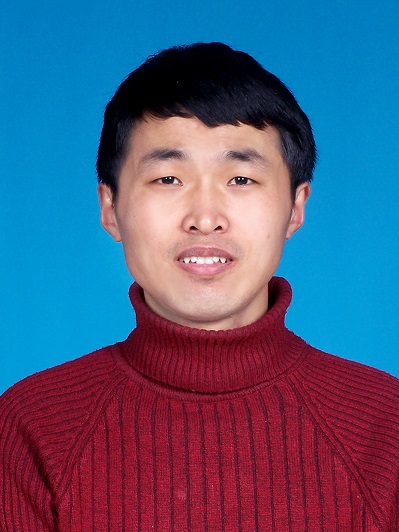
\includegraphics[height=0.7in]{Figures/Person_Photo.JPG}\\
\end{minipage}\vskip 3pt
\fontsize{9.2pt}{6.2pt}\selectfont{\textcolor{magenta}{教育背景}}
	\begin{itemize}
		\item {\fontsize{8.2pt}{6.2pt}\selectfont{\textrm{2001.09-2008.01}}}~~~北京大学~化学与分子工程学院~~~~~~物理化学
		\item {\fontsize{8.2pt}{6.2pt}\selectfont{\textrm{1997.09-2001.06}}}~{\fontsize{8.2pt}{6.2pt}\selectfont{中国纺织大学(现~东华大学)}}~{\fontsize{8.2pt}{6.2pt}\selectfont{纺织化学系~染整工程}}
	\end{itemize}
	\fontsize{9.2pt}{6.2pt}\selectfont{\textcolor{magenta}{工作简历}}
\begin{table}[!h]
\tabcolsep 0pt \vspace*{-5pt}
%\caption{经费预算表 (单位:~万元).}
\label{Table-Cost}
\begin{minipage}{\textwidth}
%\begin{center}
\centering
\def\temptablewidth{0.94\textwidth}
\renewcommand\arraystretch{2.2} %表格宽度控制(普通表格宽度的两倍)
\rule{\temptablewidth}{1pt}
\begin{tabular*} {\temptablewidth}{@{\extracolsep{\fill}}c@{\extracolsep{\fill}}c@{\extracolsep{\fill}}c}
%-------------------------------------------------------------------------------------------------------------------------
	起止时间 &工作单位	&研发岗位 \\\hline
	\fontsize{8.2pt}{6.2pt}\selectfont{\textrm{2008.01-2012.03}} &\fontsize{8.2pt}{6.2pt}\selectfont{北京大学~化学与分子工程学院} &\fontsize{8.2pt}{6.2pt}\selectfont{博士后(两期)} \\
	\fontsize{8.2pt}{6.2pt}\selectfont{\textrm{2012.03-2013.03}} &\fontsize{8.2pt}{6.2pt}\selectfont{北京宏剑公司} \fontsize{8.2pt}{6.2pt}\selectfont{&高级技术支持}\\
	\fontsize{8.2pt}{6.2pt}\selectfont{\textrm{2013.04-2016.03}} &\fontsize{7.8pt}{6.2pt}\selectfont{中物院高性能数值模拟软件中心} &\fontsize{8.2pt}{6.2pt}\selectfont{金属材料模拟团队} \\
	\fontsize{8.2pt}{6.2pt}\selectfont{\textrm{2016.04-至今}}    &\fontsize{8.2pt}{6.2pt}\selectfont{北京市计算中心} &\fontsize{8.2pt}{6.2pt}\selectfont{云平台事业部}
\end{tabular*}
\rule{\temptablewidth}{1pt}
%\end{center}
\end{minipage}
\end{table}
%\vskip -3pt
}


%\section{第一原理材料计算核心软件研究}
\frame
{
	\frametitle{第一原理材料计算核心软件性能改进研究}
	\begin{itemize}
		\item {\fontsize{7.5pt}{6.2pt}\selectfont{采用$\vec k\cdot\vec p$方法改善\textrm{WIEN2k}软件的计算效率,将计算效率提升\textrm{1-2}个数量级,使之可计算更复杂的材料物性}}
	\end{itemize}
\begin{figure}[h!]
\centering
\vskip -20pt
\subfigure[\fontsize{6.5pt}{6.2pt}\selectfont{\textrm{Band}}]{
\label{band_kp}
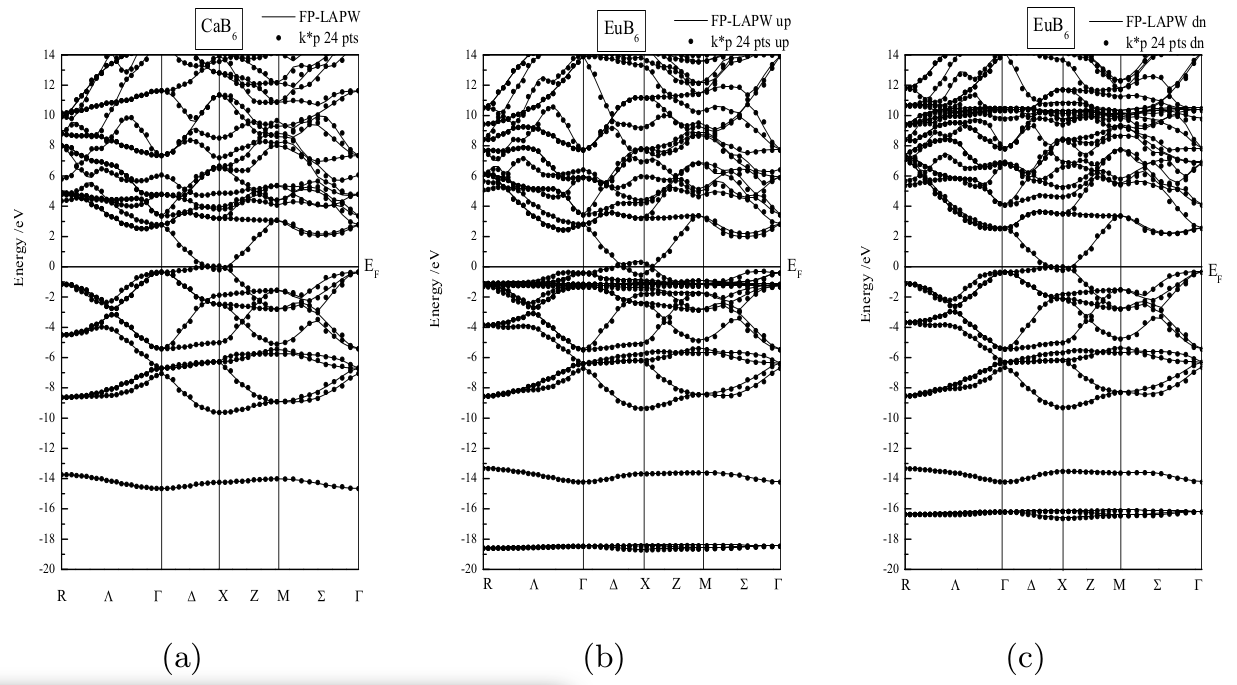
\includegraphics[height=0.9in,width=0.7in,viewport=0 50 310 560,clip]{Figures/Band_kp.png}}
\subfigure[\fontsize{6.5pt}{6.2pt}\selectfont{\textrm{Computing Time}}]{
\label{Time_kp}
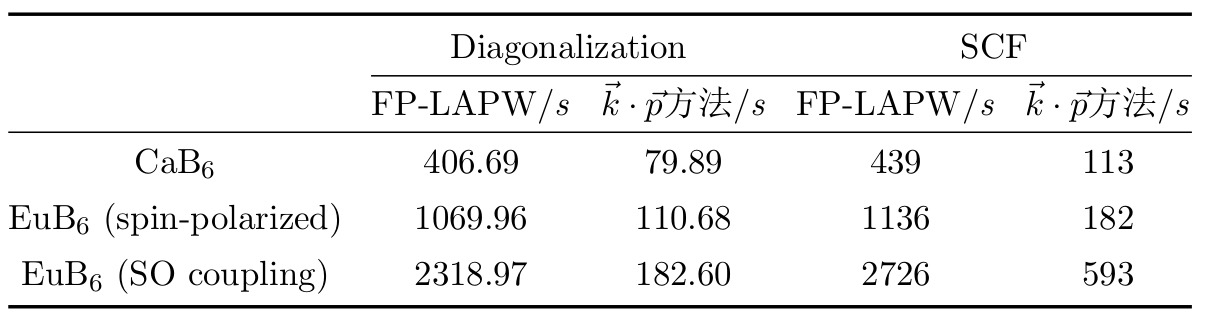
\includegraphics[height=0.6in]{Figures/Time_kp.png}}
\subfigure[\fontsize{6.5pt}{6.2pt}\selectfont{\textrm{Equation of State}}]{
\label{EOS_kp}
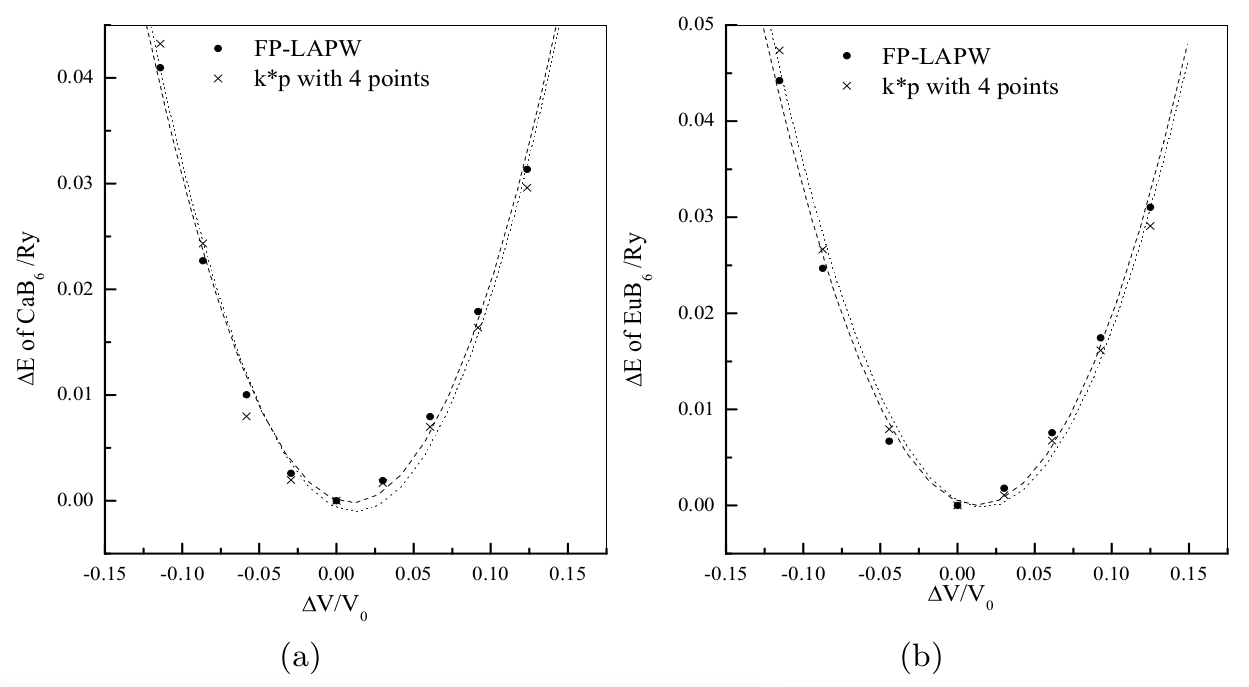
\includegraphics[height=1.0in,width=0.95in,viewport=0 50 460 560,clip]{Figures/EOS_kp.png}}
%\caption{\fontsize{6.2pt}{6.2pt}\selectfont{$\vec k\cdot\vec p$方法(点)与常规\textrm{DFT}方法计算的能带对比:\textrm{(a)CaB$_6$,(b)EuB$_6$-spin~up,\\(c)EuB$_6$-spin~dn}}}%
%\label{band_kp}
%\caption{\fontsize{5.2pt}{6.2pt}\selectfont{$\vec k\cdot\vec p$方法保证计算精度,并计算效率提升}}%
\end{figure}
\vskip -5pt
	\begin{itemize}
		\item {\fontsize{7.5pt}{6.2pt}\selectfont{基于开源软件\textrm{AtomPAW~}探索商业软件\textrm{VASP~}赝势的参数优化方案}}
	\end{itemize}
\begin{figure}[h!]
\centering
\vskip -5pt
\subfigure[\fontsize{6.5pt}{6.2pt}\selectfont{\textrm{FCC-Al}}]{
\label{FCC-Al-PAW}
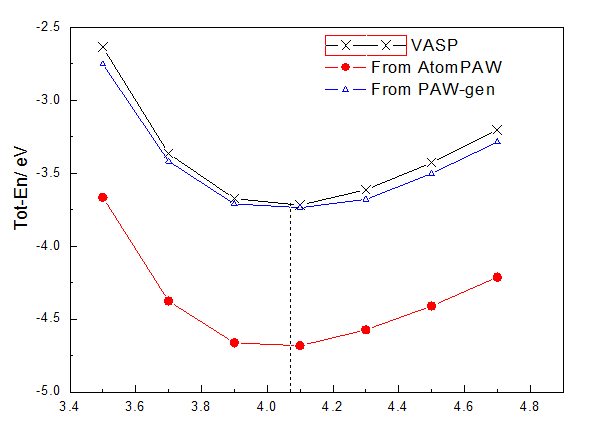
\includegraphics[height=0.8in]{Figures/CAEP-SCNS-14.png}}
\subfigure[\fontsize{6.5pt}{6.2pt}\selectfont{\textrm{FCC-Cu}}]{
\label{FCC-Cu_PAW}
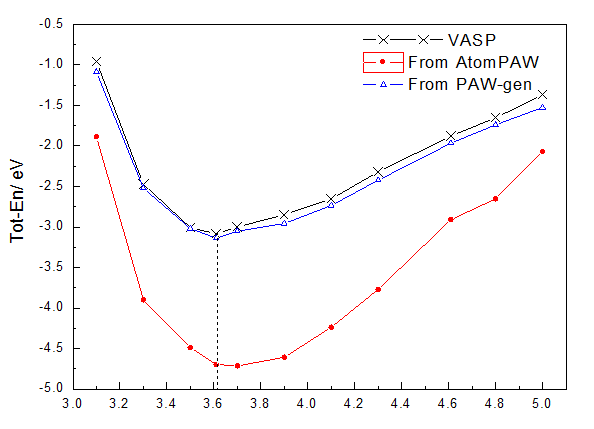
\includegraphics[height=0.8in]{Figures/CAEP-SCNS-15.png}}
\subfigure[\fontsize{6.5pt}{6.2pt}\selectfont{\textrm{HCP-Zr}}]{
\label{HCP-Zr_PAW}
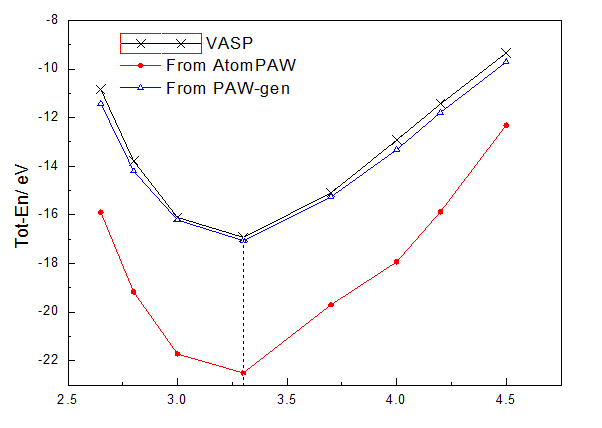
\includegraphics[height=0.8in]{Figures/CAEP-SCNS-16.png}}
%\caption{\fontsize{7.5pt}{6.2pt}\selectfont{不同金属的\textrm{E-V}曲线与\textrm{VASP}计算结果对比}}%
%\label{band_kp}
\end{figure}
}

%\section{高通量材料计算自动流程软件开发}
\frame
{
	\frametitle{适应复杂原子间相互作用势高通量计算流程开发}
\begin{itemize}
	\setlength{\itemsep}{1pt}
	\item {\fontsize{8.2pt}{4.2pt}\selectfont{\textcolor{purple}{高温合金材料}:~微观原子间相互作用决定体系的宏观力学性质}}
	\item {\fontsize{8.0pt}{4.2pt}\selectfont{\textcolor{purple}{催化活性材料}:~与反应物间相互作用强弱,直接影响材料的催化性能}}
\end{itemize}
\begin{minipage}[b]{0.49\linewidth}
	\begin{itemize}
		\item \fontsize{8.0pt}{4.2pt}\selectfont{国内外现有自动流程软件概况}
	\end{itemize}
\begin{table}[!h]
\tabcolsep 0pt \vspace*{-12pt}
%\caption{}
\label{Table-Cost}
\begin{minipage}{\textwidth}
%\begin{center}
\centering
\def\temptablewidth{1.1\textwidth}
\renewcommand\arraystretch{0.8} %表格宽度控制(普通表格宽度的两倍)
\rule{\temptablewidth}{1pt}
\begin{tabular*} {\temptablewidth}{@{\extracolsep{\fill}}c@{\extracolsep{\fill}}c@{\extracolsep{\fill}}c@{\extracolsep{\fill}}c@{\extracolsep{\fill}}c@{\extracolsep{\fill}}c@{\extracolsep{\fill}}c}
%-------------------------------------------------------------------------------------------------------------------------
	&\multirow{2}{*}{\fontsize{5.2pt}{4.2pt}\selectfont{编程语言}}	&\fontsize{5.2pt}{4.2pt}\selectfont{建模} &\multicolumn{2}{|c|}{\fontsize{4.2pt}{3.2pt}\selectfont{任务提交与管理}} &\multirow{2}{*}{\fontsize{5.2pt}{4.2pt}\selectfont{后处理}} &\multirow{2}{*}{\fontsize{4.2pt}{3.2pt}\selectfont{数据组织管理}} \\\cline{4-5}
	&	&\fontsize{5.2pt}{4.2pt}\selectfont{功能} &\multicolumn{1}{|c|}{\fontsize{5.2pt}{4.2pt}\selectfont{软件接口}} &\multicolumn{1}{c|}{\fontsize{5.2pt}{4.2pt}\selectfont{运行容错}} & & \\\hline
	\fontsize{5.2pt}{4.2pt}\selectfont{{AFLOW}} &\fontsize{5.2pt}{4.2pt}\selectfont{C++} &\checkmark &\triangle &\FiveStarOpen &\FiveStarOpen &\fontsize{5.2pt}{4.2pt}\selectfont{{Django}} \\
	\fontsize{5.2pt}{4.2pt}\selectfont{{MP}} &\fontsize{5.2pt}{4.2pt}\selectfont{Python} &\checkmark &\checkmark &\FiveStarOpen &\FiveStarOpen &\fontsize{5.2pt}{4.2pt}\selectfont{{MongoDB}} \\
	\multirow{2}{*}{\fontsize{5.2pt}{4.2pt}\selectfont{{QMIP}}} &\fontsize{5.2pt}{4.2pt}\selectfont{JavaScript/SVG} &\multirow{2}{*}{\checkmark} &\multirow{2}{*}{\checkmark} &\multirow{2}{*}{--} &\multirow{2}{*}{\checkmark} &\multirow{2}{*}{--} \\
	&\fontsize{5.2pt}{4.2pt}\selectfont{+html/Python} & & & & & \\
	\fontsize{5.2pt}{4.2pt}\selectfont{{CEP}} &\fontsize{5.2pt}{4.2pt}\selectfont{Python} &\checkmark &\checkmark &-- &\checkmark &\fontsize{5.2pt}{4.2pt}\selectfont{{Django/MySQL}} \\
	\fontsize{5.2pt}{4.2pt}\selectfont{{ASE}} &\fontsize{5.2pt}{4.2pt}\selectfont{Python} &\FiveStarOpen &\FiveStarOpen &-- &\triangle &-- \\
	\multirow{2}{*}{\fontsize{5.2pt}{4.2pt}\selectfont{{MatCloud}}} &\fontsize{5.2pt}{4.2pt}\selectfont{JavaScript} &\multirow{2}{*}{\checkmark} &\multirow{2}{*}{\triangle} &\multirow{2}{*}{\checkmark} &\multirow{2}{*}{\checkmark} &\multirow{2}{*}{\fontsize{5.2pt}{4.2pt}\selectfont{{MongoDB}}} \\
	&\fontsize{5.2pt}{4.2pt}\selectfont{+.NETCore} & & & & &
\end{tabular*}
\rule{\temptablewidth}{1pt}
\end{minipage}
\vskip -15pt
\fontsize{4.2pt}{3.2pt}\selectfont{
\begin{description}
	\item[\FiveStarOpen]~该功能较突出
	\item[\checkmark]~该功能基本满足需求
	\item[\triangle]~该功能存在不足
\end{description}}
%\end{center}
\end{table}
\end{minipage}
\hfill
\begin{minipage}[b]{0.49\linewidth}
	\begin{itemize}
		\item \fontsize{8.0pt}{4.2pt}\selectfont{适用于异质界面的高通量材料计算自动流程软件架构}
\begin{figure}[h!]
\centering
\vskip -12pt
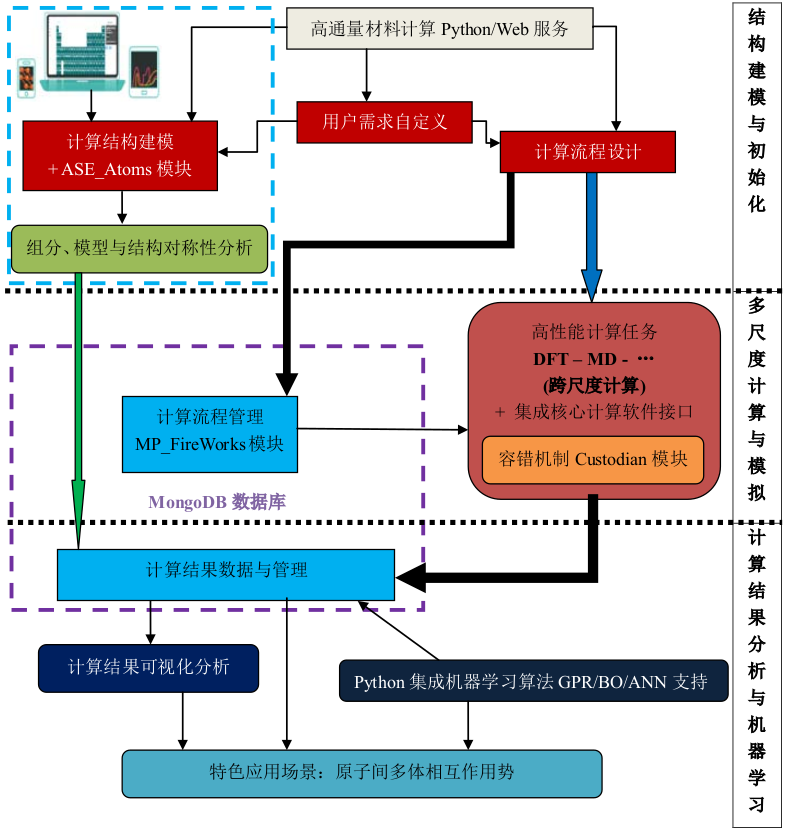
\includegraphics[height=2.18in]{Figures/MP_comp_BCC.png}
%\caption{\fontsize{6.5pt}{4.2pt}\selectfont{适应多体相互作用的高通量计算流程结构示意}}%
\label{MP_comp_BCC}
\end{figure}
	\end{itemize}
\end{minipage}
}

\frame
{
	\frametitle{数据库支持的材料计算自动流程与能带表示标准化}
	\begin{itemize}
		\item {\fontsize{8.2pt}{4.2pt}\selectfont{将材料计算流程分解为基本计算任务,\textcolor{purple}{通过数据库技术组织成有序的计算工作流},实现复杂材料计算流程自动化}}
\begin{figure}[h!]
\centering
\vskip -5pt
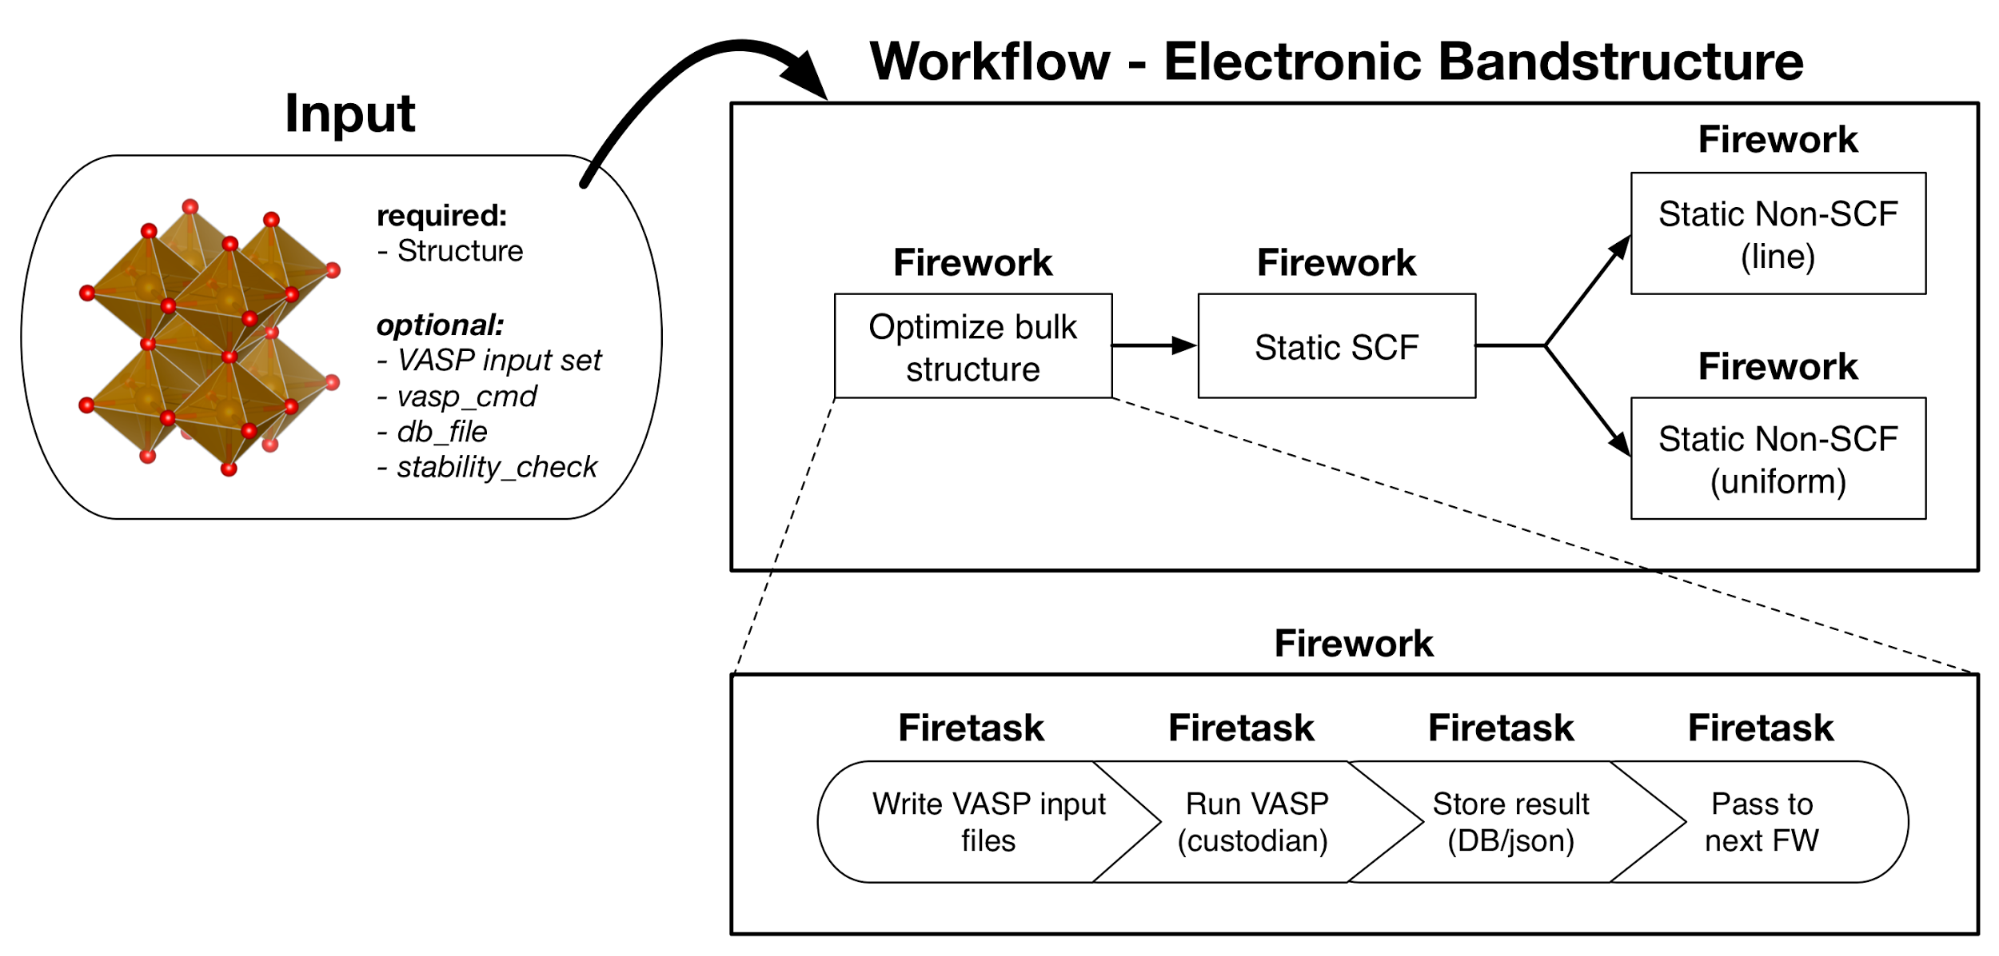
\includegraphics[height=1.1in]{Figures/bandstructure_wf.png}
%\caption{\fontsize{7.2pt}{}\selectfont{\textrm{Anatomy of a band structure workflow consisting of 4 separate calculations (Fireworks).}}}%
\label{bandstructure_wf}
\end{figure}
		\item {\fontsize{8.0pt}{4.2pt}\selectfont{材料计算自动流程和电子结构分析需求,\textcolor{purple}{驱动能带表示~$\vec k$-\textrm{path}“标准化”}}}
\begin{figure}[h!]
\centering
\vspace*{-0.1in}
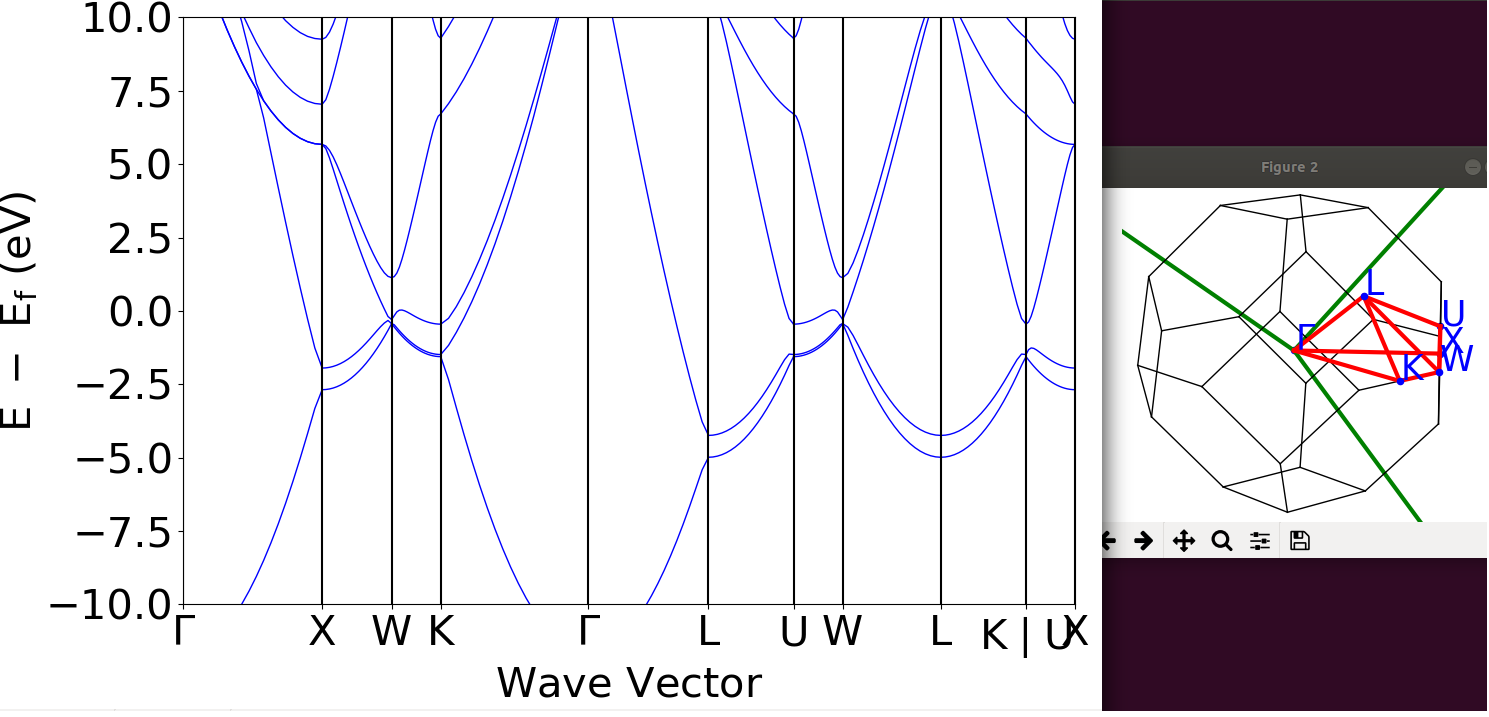
\includegraphics[height=1.15in,width=2.5in,viewport=0 0 1150 560,clip]{Figures/FCC_Si-k-path.png}
%\caption{\fontsize{7.2pt}{4.2pt}\selectfont{\textrm{The Band-structure of FCC-Si with standard $\vec k$-path selection.}}}%
\label{FCC-Si_bandstruct}
\end{figure} 
	\end{itemize}
}

\frame
{
	\frametitle{技术服务与推广应用}
	\begin{itemize}
		\setlength{\itemsep}{15pt}
		\item 多次组织和主讲“第一原理材料计算方法与软件”培训课程
		\item 课程涵盖第一原理材料计算基础理论、计算方法、程序算法和软件结构,主要包括:\vskip 5pt
			{\fontsize{8.5pt}{4.2pt}\selectfont{密度泛函基本理论、固体能带理论}}\vskip 5pt
			{\fontsize{8.5pt}{4.2pt}\selectfont{赝势-平面波方法、\textrm{LAPW~}方法、\textrm{PAW~}方法}}\vskip 5pt
			{\fontsize{8.5pt}{4.2pt}\selectfont{$\vec k$-空间积分方法、电子相关与磁性(\textrm{LDA+}\textit{U}方法)}}\vskip 5pt
			{\fontsize{8.5pt}{4.2pt}\selectfont{\textrm{WIEN2k}/\textrm{ELK}/{\textrm{VASP}/\textrm{ABINIT}等软件结构与使用}}}
		\item 课程面向国内高校物理、化学与材料专业的研究生和青年教师,已有超过百余人参加培训
	\end{itemize}
}

\appendix
\frame
{
	\frametitle{学术积累}
\textcolor{magenta}{发表论文}
	\begin{itemize}
		\item {\fontsize{5.2pt}{1.2pt}\selectfont{\textrm{Yang Ge, Jianlong Ji, Zhizhong Shen, Qiang Zhang, Aoqun Jian, Qianqian Duan, Chao Wang, \underline{Jun Jiang}, Wendong Zhang, Shengbo Sang, First principles study of magnetism induced by topological frustration of bowtieshaped graphene nanoflake, \textit{Carbon}, \textbf{127}, (2018), 432-436}}}
		\item {\fontsize{5.2pt}{1.2pt}\selectfont{\textrm{\underline{JIANG Jun}, BIAN Jiang; LI Le-Min, Theoretical Assignments of the Optical Conductivity and Energy-loss Function Spectra of EuB$_6$, \textit{Acta Physico-Chimica Sinica}, \textbf{24}, (2008), 1-7}}}
	\end{itemize}
\textcolor{magenta}{承担和参与课题}
\begin{itemize}
	\setlength{\itemsep}{5pt}
	\item {\fontsize{8.2pt}{6.2pt}\selectfont{国家重点研发计划项目}}{\fontsize{8.2pt}{4.2pt}\selectfont{(编号:~\textrm{2017YFB0701500})}}\\
		“高通量并发式材料计算算法和软件”{\fontsize{8.2pt}{6.2pt}\selectfont{(本单位任务责任人)}}
	\item {\fontsize{8.2pt}{6.2pt}\selectfont{北科院青年骨干计划项目}}{\fontsize{8.2pt}{4.2pt}\selectfont{(编号:~\textrm{YC201820})}}\\
“基于甲烷催化燃烧机理的材料计算自动流程设计”{\fontsize{8.2pt}{6.2pt}\selectfont{(负责)}}
	\item {\fontsize{8.2pt}{6.2pt}\selectfont{国家重点研发计划项目}}{\fontsize{8.2pt}{4.2pt}\selectfont{(编号:~\textrm{2017YFB0704302})}}\\
“材料高通量计算/实验平台数据自动汇交技术”{\fontsize{8.2pt}{6.2pt}\selectfont{(参与)}}
\end{itemize}
}
%-----------------------------------------------------------Beamer下不建议使用bib,因为涉及分页--------------------------------------------------------------------------%
\begin{thebibliography}{99}
%-----------------------------------------------------------------------------------------------------------------------------------------------------------------------%
%\frame
%{
%\frametitle{主要参考文献}
%\fontsize{7.5pt}{3.9pt}\selectfont{
%	\bibitem{CMS58-227_2012}\textrm{S. Curtarolo, W. Setyawan, S. Wang, J. Xue, K. Yang, R. H. Taylor, L. J. Nelson, G. L. Hart, S. Sanvito, M. Buongiorno-Nardelli, N. Mingo and O. Levy. \textit{Comp. Mater. Sci.}, \textbf{58} (2012), 227}
%	\bibitem{CMS97-209_2015}\textrm{S. P. Ong, S. Cholia, A. Jain, M. Brafman, D. Gunter, G. Ceder and K. A. Persson. \textit{Comp. Mater. Sci.}, \textbf{97} (2015), 209}
%	\bibitem{url_QMIP}\textrm{\url{http://www.qmip.org/qmip.org/Welcome.html}}
%	\bibitem{JPCL2-2241_2011}\textrm{J. Hachmann, R. Olivares-Amaya, S. Atahan-Evrenk, C. Amador-Bedolla, R. S. S$\acute{a}$nchez-Carrera, A. Gold-Parker, L. Vogt, A. M. Brockway and A. Aspuru-Guzik. \textit{J. Phys. Chem. Lett.}, \textbf{2} (2011), 2241}
%	\bibitem{JPCM29-273002_2017}\textrm{A. H. Larsen, J. J. Mortensen, J. Blomqvist, I. E. Castelli, R. Christensen, M. Du{\l}ak, J. Friis, M. N. Groves, B. Hammer, C. Hargus, E. D. Hermes, P. C. Jennings, P. B. Jensen, J.Kermode, J. R. Kitchin, E. L. Kolsbjerg, J. Kubal, K. Kaasbjerg, S. Lysgaard, J. B. Maronsson, T. Maxson, T. Olsen, L. Pastewka, A. Peterson, C. Rostgaard, J. Schi{\o}tz, O. Sch\"utt, M. Strange, K. S. Thygesen, T. Vegge, L. Vilhelmsen, M. Walter, Z. Zeng, K. W. Jacobsen. \textit{J. Phys.:~ Condens. Matter.}, \textbf{29} (2017), 273002}
%	\bibitem{CMS146-319_2018}\textrm{X. Yang, Z. Wang, X. Zhao, J. Song, M. Zhang, H. Liu. \textit{Comp. Mater. Sci.}, \textbf{146} (2018), 319}
%}
%}
%\nocite*{}
%}

%\frame
%{
%\frametitle{发展统一理论框架下的材料计算程序}
%\begin{itemize}
%	\item
%\end{itemize}
%}


%{\small
%\phantomsection\addcontentsline{toc}{section}{Bibliography}	 %直接调用\addcontentsline命令可能导致超链指向不准确,一般需要在之前调用一次\phantomsection命令加以修正	%
%\bibliography{Myref}																			%
%\bibliographystyle{mybib}																		%
%  \nocite{*}																				%
%}

%------------------------------------------------------------------------------------------------------------------------------------------------------------------------------%


%-------------------------------------------------------------------------Thanks------------------------------------------------------------------------------------------------
%\section{致谢}
%\frame
%{
%\frametitle{致$\quad$谢}
%\begin{itemize}
%    \setlength{\itemsep}{20pt}
%  \item 感谢本团队高兴誉、吴泉生、宋红州等各位老师参与的讨论
%  \item 感谢莫所长、宋主任以及软件中心各位老师和同事
%  \item 感谢王崇愚先生的帮助
%\end{itemize}
%}

%-------------------------------------------------------------------------------------------------------------------------------------------------------------------------------

%\begin{thebibliography}{99}
%-----------------------------------------------------------------------------------------------------------------------------------------------------------------------%
%\frame
%{
%\frametitle{主要参考资料}
%	\bibitem{Origin-1}网络流传资料:~\textrm{Origin~}图形绘制及曲线拟合.ppt\\{\footnotesize\url{https://wenku.baidu.com/view/7e7c775de2bd960591c67705.html}}					%
%	\bibitem{Origin-2}网络流传资料:~\textrm{Origin~}图形绘制基础入门及曲线拟合.ppt\\{\footnotesize\url{https://wenku.baidu.com/view/d2b85773f46527d3240ce05e.html}}					%
%	\bibitem{Origin-3}网络流传资料:~{\textit{方东明}},~\textrm{Origin~8.0~}二维图形绘制制详解实例和教程.pdf\\{\footnotesize\url{https://wenku.baidu.com/view/eaf64026bd64783e09122b66.html}}					%
%	\bibitem{Origin-4}\textrm{Origin~}官网视频教程:\\{\footnotesize\url{http://www.originlab.com/index.aspx?go=SUPPORT/VideoTutorials}}					%
%	\bibitem{Matlab-1}网络流传资料:~\textrm{Matlab~}绘制曲线的方法.ppt\\{\footnotesize\url{https://wenku.baidu.com/view/dad6257a02768e9951e738e1.html}}					%
%\nocite*{}
%}

%\frame
%{
%\frametitle{发展统一理论框架下的材料计算程序}
%\begin{itemize}
%	\item
%\end{itemize}
%}


%-----------------------------------------------------------Beamer下不建议使用bib,因为涉及分页--------------------------------------------------------------------------%
%{\small
%\phantomsection\addcontentsline{toc}{section}{Bibliography}	 %直接调用\addcontentsline命令可能导致超链指向不准确,一般需要在之前调用一次\phantomsection命令加以修正	%
%\bibliography{Myref}																			%
%\bibliographystyle{mybib}																		%
%  \nocite{*}																				%
%}

%------------------------------------------------------------------------------------------------------------------------------------------------------------------------------%


%-------------------------------------------------------------------------Thanks------------------------------------------------------------------------------------------------
%\section{致谢}
%\frame
%{
%\frametitle{致$\quad$谢}
%\begin{itemize}
%    \setlength{\itemsep}{20pt}
%  \item 感谢本团队高兴誉、吴泉生、宋红州等各位老师参与的讨论
%  \item 感谢莫所长、宋主任以及软件中心各位老师和同事
%  \item 感谢王崇愚先生的帮助
%\end{itemize}
%}

\logo{}									%不显示logo
%\frame
%{
%\vskip 60 pt
%%\hskip 10pt \textcolor{blue}{\Huge 感谢答辩委员会各位老师\,\textrm{!}}\\
%\vskip 35 pt
%\hskip 60pt \textcolor{blue}{\fontsize{46.2pt}{6.2pt}\selectfont{谢谢大家\:!}}
%\vskip 15 pt
%\hskip 40pt \textcolor{blue}{\Huge \textrm{for your attention\:!}}
%}

%-------------------------------------------------------------------------------------------------------------------------------------------------------------------------------

\clearpage
%\end{CJK*}
\end{document}
